\documentclass[]{scrartcl}
\usepackage{graphicx}


\title{Airborne sound isolation homework}
\date{Room Acoustics - Music and Acoustic Engineering -Politecnico di Milano}
\author{Lercari Mattia 10751919, Lampis Alessio 10743504}
\subtitle{01/11/2020 - Academic year 2020/2021}

\begin{document}
\maketitle

\section{Calculate the sound reduction index of each components}
\subsection{Facades}
The material that has been chosen to design facades of the room under study is lightweight concrete. Walls have thickness of $300$ mm and its sound reduction indexes (dB) are shown in following table. 
\begin{tabular}{|c|c|c|c|c|c|c|}
	\hline
	63 Hz & 125 Hz & 250 Hz & 500 Hz & 1000 Hz & 2000 Hz & 4000 Hz \\
	\hline
	37 & 37 & 42 & 51 & 58 & 58 & 58 \\
	\hline
\end{tabular} Since they are evaluated in octave bands, it is needed to interpolate linearly values in third octave bands so that can be used in Excel file we reference. Linear interpolation is calculated using 
\begin{equation}
	R_f = R_{f1} + \frac{f - f_1}{f_2 - f_1}(R_{f2} - R_{f2}). \quad \quad  f_1<f<f_2
\end{equation} where $R_{fi} = R(f_i)$ indexes are refered to frequencies in third octave bands. The result can be found in "facade wall" sheet. Moreover, its areic mass is $m'= 390 $ $ Kg/m^2$. From the table, as well as from the Excel computations, the weighted sound reduction index is $R_w = 54$ and correction coefficients $C$ and $C_{tr}$ are $-2$ and $-6$, respectively. 
\subsection{Windows}

\begin{figure}[h]
	\centering
	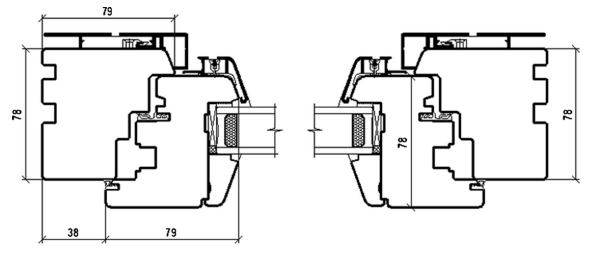
\includegraphics[width=0.7\linewidth]{windows_profile}
	\caption{Horizontal cross section of tested window}
	\label{fig:windowsprofile}
\end{figure}


Sound reduction indexes of windows come from a scientific paper \cite{Window}.The measurements of the experimental study were done in one third octave bands from 100 Hz to 5000 Hz according to LST EN ISO 10140 series standards. Measurements results were evaluated according to LST EN ISO 717-1 standard. The glass we chose it is named WOG2/1 in the paper, it is made of two layers of ordinary glass (4 mm and 6 mm) with a 18 mm of argon gas in between. Since the paper doesn't provide any information about material density, we used a common value of soda lime glass density, $ \rho = 2530$ $Kg/m^3$. The corresponding areic mass is $m' = 25.3$ $Kg/m^3$.
In following figure it is shown sound reduction indexes for WOG2/1.  Here $R_w$ evaluated in the Excel and the one which can be found in the paper are coincident, while coefficients $C$ and $C_{tr}$ are $-2$ and $-6$ in our computation but $-1$ and $-5$ according to the cited study. 

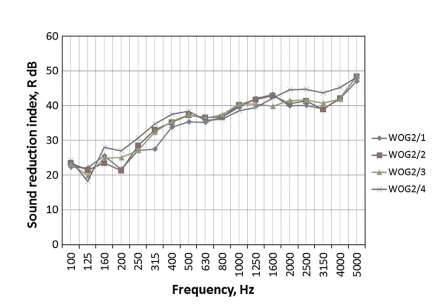
\includegraphics[width=0.7\linewidth]{windows_sound_reduction}

\subsection{Floor and ceiling}
From table of material we chose $240$ mm of Ca-Si blocks as construction which has a remarkable areic mass ($420$ $Kg/m^2$) and no linear interpolation was computed because "floor" and "ceiling" sheets in our Excel are based on one octave bands subdivision. Reduction indexes are \begin{tabular}{|c|c|c|c|c|c|c|}
	\hline
	63 Hz & 125 Hz & 250 Hz & 500 Hz & 1000 Hz & 2000 Hz & 4000 Hz \\
	\hline
	38 & 38 & 46 & 54 & 62 & 68 & 68 \\
	\hline
\end{tabular}

The weighted value given by table is $56$ while it is $57$ in the Excel, as well as correction coefficients are $-1,-6$ in the table while $-2,-7$ in the sheets. 

\subsection{Internal walls}
From the catalogue of an italian company called FOROSON we found results of measurement realized on their bricks. It has been taken a FOROSON brick with plaster and a total thickness of $33$ cm. Isolation properties were studied according to UNI EN ISO 140-4, $R_w'$ has been calculated following the UNI EN ISO 717-1 and since we used the same standards, our indexes are the same of the catalogue (see figure \ref{fig:poroton} ).
\begin{figure}[h]
	\centering
	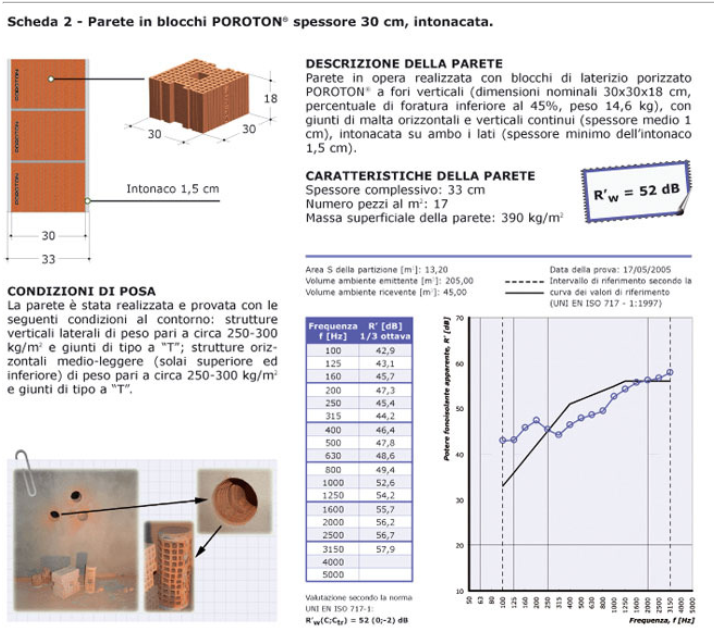
\includegraphics[width=0.9\linewidth]{poroton}
	\caption{Poroton results on plastered brick wall}
	\label{fig:poroton}
\end{figure}

\subsubsection{Door}
Since we wanted to have a wooden door but keep an high sound reduction index compared to the second homework, we decided to use one of the most heavy wood, the ITIS (Prosopis kuntzei). "This small South American tree could be considered a super-mesquite. Related to mesquite, it’s very dark, very dense, and very hard; a good substitute for ebony" \cite{wood}. Its density is $\mathit{1275 Kg/m^3}$ and we designed two layers of $\mathit{1 cm}$ of wood and a $\mathit{4 cm}$ of rockwool in between. Having these parameters and assuming a diffusive sound propagation through the door, we applied the mass law and obtained $R_w'= 40 dB (-4, -12)$. 

\section{Verify the passive acoustic requirements of buildings}  

In the Excel, section "data", are resumed sound absorption of each component between room A and room B given by direct and flanking contributions. In section "joints" are computed  vibration reduction index for each junction. The main result is the total weighted sound reduction index between room that is  $50,29$ $dB$, above the legal threshold of $50$ $dB$ (D.P.C.M 5-12-1997) as well as the facade sound reduction index, which is $53.3$ $dB$. 


\end{document}
